\documentclass[10pt]{article}
\usepackage[hmargin={.5in},vmargin={.5in},foot={.6in}]{geometry}   
\geometry{letterpaper}              
\usepackage{color,graphicx}
\usepackage{setspace}
\usepackage{amsmath}
\usepackage{amssymb}
\usepackage{varioref}
\usepackage{textcomp}
\usepackage{textcomp}
\usepackage{mflogo}
\usepackage{wasysym}
\usepackage[normalem]{ulem}
\usepackage{hyperref}
\usepackage{booktabs}
\usepackage{natbib}
\usepackage{linguex}
\usepackage{qtree}

\qtreecenterfalse

\newcommand{\HRule}{\rule{\linewidth}{0.25mm}}

\usepackage{fancyhdr} % This should be set AFTER setting up the page geometry
\pagestyle{plain} % options: empty , plain , fancy
\lhead{}\chead{}\rhead{}
\renewcommand{\headrulewidth}{.5pt}
\lfoot{}\cfoot{\thepage}\rfoot{}
\newcommand{\txtp}{\textipa}
\renewcommand{\rm}{\textrm}
\newcommand{\sem}[1]{\mbox{$[\![$#1$]\!]$}}
\newcommand{\lam}{$\lambda$}
\newcommand{\lan}{$\langle$}
\newcommand{\ran}{$\rangle$}
\newcommand{\type}[1]{\ensuremath{\left \langle #1 \right \rangle }}

\newcommand{\bex}{\begin{exe}}
\newcommand{\eex}{\end{exe}}
\newcommand{\bit}{\begin{itemize}}
\newcommand{\eit}{\end{itemize}}
\newcommand{\ben}{\begin{enumerate}}
\newcommand{\een}{\end{enumerate}}

\newcommand{\gcs}[1]{\textcolor{blue}{[gcs: #1]}}


\thispagestyle{plain}

\begin{document}

%\maketitle

\begin{center}
	\textbf{On the role of conjunction in adjective ordering preferences}
\end{center}
Adjective ordering preferences are robustly attested in English and many unrelated languages \citep{dixon1982,sproatshih1991,scontrasetal2017adjectives}. In nominals with multi-adjective strings (e.g., \emph{big blue box}), chances are the order of the adjectives is non-arbitrary. However, ordering preferences are claimed to neutralize in cases where multi-adjective strings are formed via conjunction (e.g., \emph{blue \uline{and} big box}; \citealp{fordolson1975,byrne1979}). We provide empirical evidence in support of this claim, but with an important caveat: conjunction neurtralizes adjective ordering preferences \emph{in languages where multi-adjective strings obligatorily feature conjunction}. %In languages where multi-adjective strings optionally feature conjunction, the regularity introduced in conjunction-less strings can bleed over to strings with conjunction.%The current study investigates the effects of conjunction on adjective ordering preferences in Spanish, a language where multi-adjective strings obligatorily feature conjunction. We then compare the Spanish results with English, where multi-adjective strings optionally feature conjunction.

In Spanish, multi-adjective strings are post-nominal and formed via conjunction (e.g., \emph{la caja grande \uline{y} azul} `the big blue box'). To investigate the status of adjective ordering preferences in Spanish, we replicated the methodology of Expt.~1: \emph{Ordering preferences} from \cite{scontrasetal2017adjectives} using Spanish translations of the original English materials. 48 native speakers indicated their preferences for pairs of multi-adjective strings that differed in the relative order of the adjectives.  Adjectives came from seven semantic classes and were paired with ten unique nouns. On the basis of the preference ratings, we calculated each adjective's preferred distance from the modified noun. Fig.~1 plots the preferred distance measures grouped by lexical semantic class for Spanish (blue bars), as well as the English baseline from \citeauthor{scontrasetal2017adjectives} (red bars). Whereas English has stable ordering preferences, as evidenced by the significant deviation from chance level (i.e., from 0.5), Spanish does not: in all but one of the lexical classes (i.e., \emph{quality}), participants fail to provide systematic ratings that would evidence stable ordering preferences; we find a similar pattern of responses at the level of individual adjectives. We then re-ran the English ordering preferences experiment  from \citeauthor{scontrasetal2017adjectives}, this time using conjunction to form the multi-adjective strings. The results from 59 English speakers are plotted in Fig.~1 (green bars); the English conjunction ratings replicate both the qualitative and quantitative results from the \citeauthor{scontrasetal2017adjectives} baseline.

Starting with Spanish, one might think that post-nominal adjectives were to blame for the absence of stable ordering preferences, but stable preferences have been documented in languages with post-nominal adjectives that do not require conjunction in multi-adjective strings (e.g., Indonesian; \citealp{martin1969competence}). Rather, it would seem that conjunction does indeed neutralize ordering preferences. This effect makes sense if the pressure for ordering preferences comes from a desire to compose less subjective adjectives earlier with the modified noun (cf.~\citealp{scontrasetal2017adjectives}); with conjunction (Fig.~2a), the adjectives make their semantic contribution together after they are conjoined, so pressures mediating the order in which adjectives compose cannot apply. 
But in English we find no measureable effect of conjunction. One way to understand this result is that in languages where multi-adjective strings optionally feature conjunction, the regularity introduced in conjunction-less strings can bleed over to strings with conjunction. English speakers seem to internalize the statistical ordering regularity from non-conjoined adjective strings and use that knowledge to inform preferences for conjoined strings.\\


\noindent\begin{minipage}[t]{.73\textwidth}
	\vspace{-9pt}
	\begin{center}	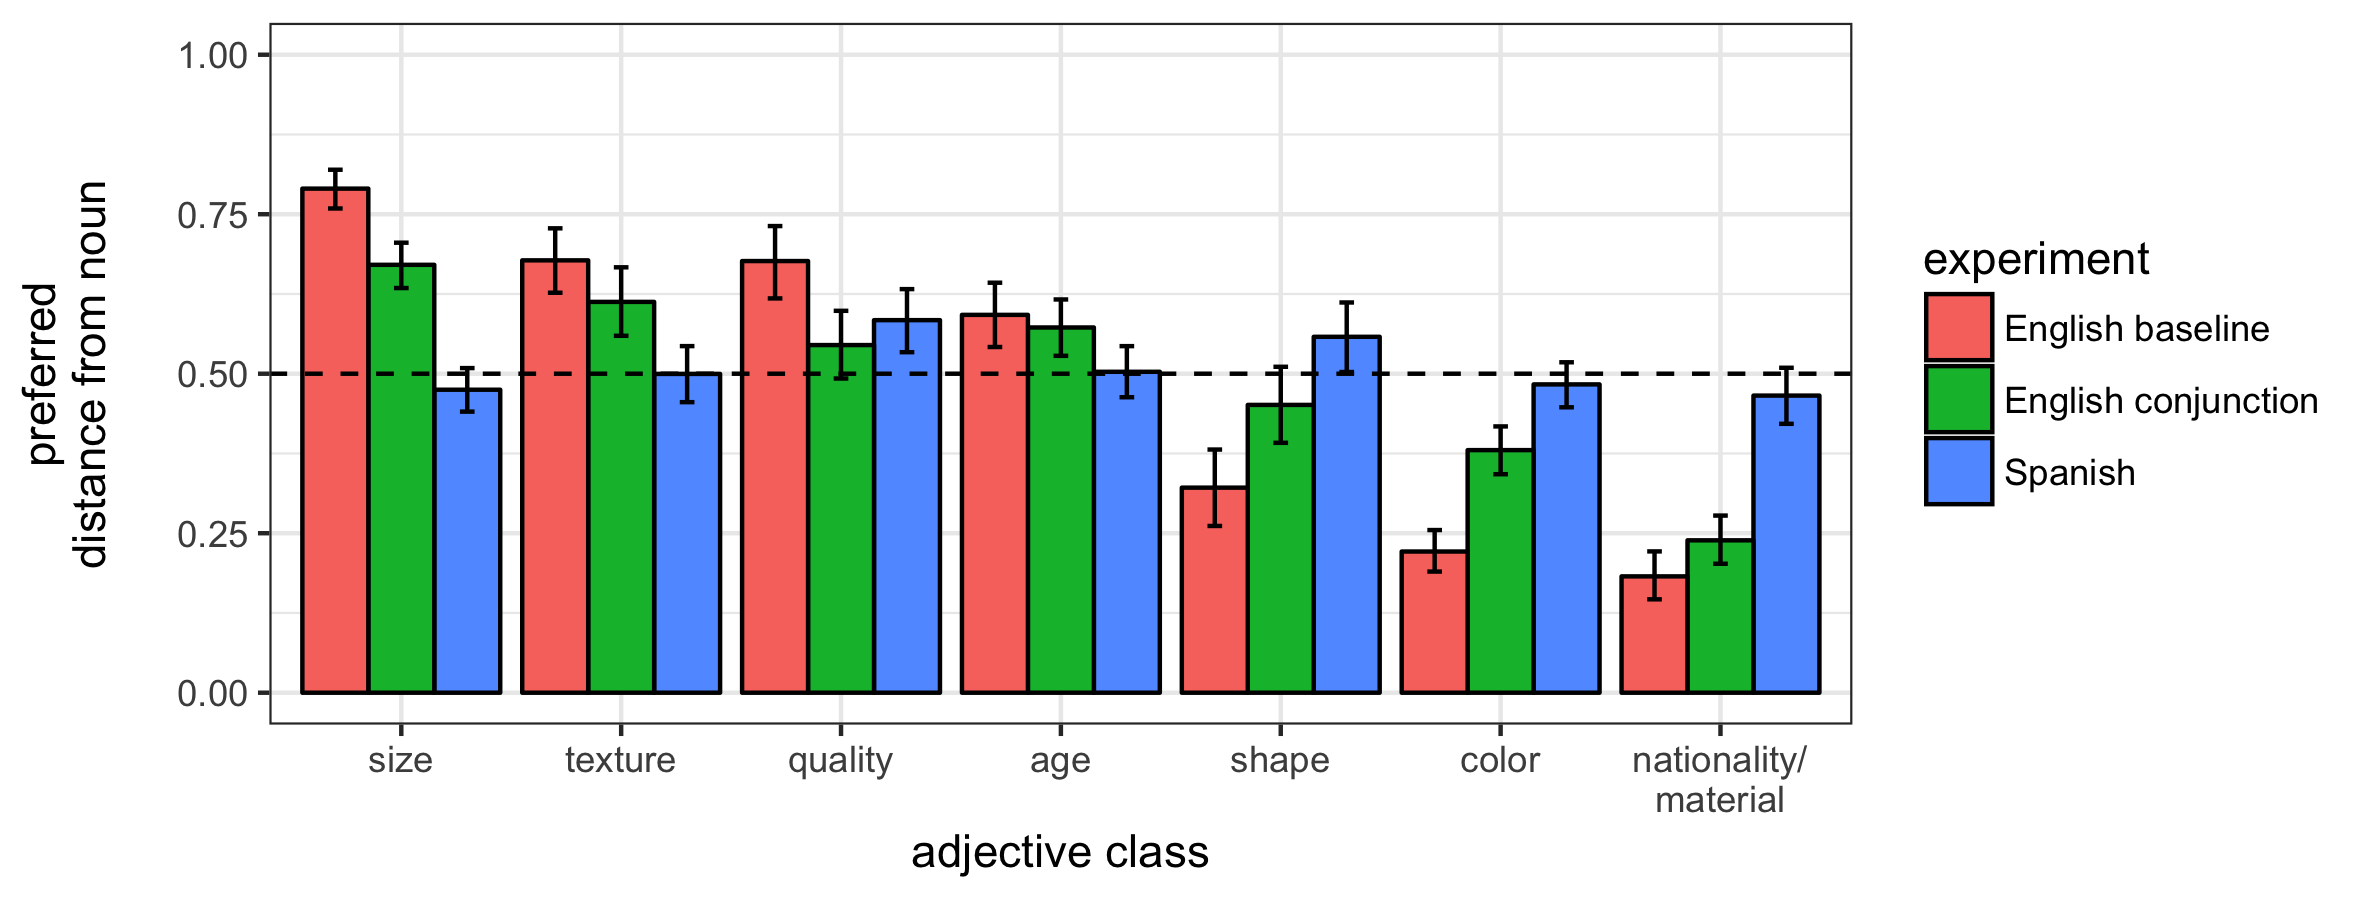
\includegraphics[width=5.6in]{../../experiments/3-order-preference-expanded2/results/LSA-class-distance.eps}
	\end{center}
	\vspace{-10pt}
	Fig.~1: Ordering preferences grouped by adjective semantic class. Higher values indicate that a class's adjectives are preferred farther from the modified noun; lower values indicate that a class's adjectives are preferred closer. The dashed line indicates chance level, or the absence of stable preferences. Error bars represent bootstrapped 95\% confidence intervals drawn from 10,000 samples of the data. Stable preferences are observed in English, both with (green bars) and without (red bars) conjunction, but not in Spanish (blue bars).
\end{minipage}
\hspace{5pt}
\begin{minipage}[t]{.24\textwidth}
	%\vspace{-85pt}
		\mbox{a.  \Tree [. [. \emph{big} [. \emph{and} \emph{blue} ] ] \emph{box} ] 	}\\	

		\mbox{b. \Tree [. \emph{big} [. \emph{blue} \emph{box} ] ] } \\
		
	Fig.~2: Compositional structure for adjective strings formed with (a) and without (b) conjunction. Only in (b) do the adjectives incrementally compose with the resulting nominal; in (a), the adjectives first get conjoined, then jointly modify the noun. % together, at the same time.
\end{minipage}


%From English to Hungarian to Mokilese, speakers exhibit strong ordering preferences in multi-adjective strings: ``the big blue box'' sounds far more natural than ``the blue big box.'' We show that an adjective's distance from the modified noun is predicted by the adjective's meaning: less subjective adjectives occur closer to the nouns they modify.  
%Subjectivity synthesizes---rather than supplants---many of the previous approaches to adjective ordering, incorporating notions like ``inherentness'' and ``context dependence'' into an intuitive psychological construct that readily operationalizes as a behavioral measure. 
%	We established two empirical constructs: first, the preferences themselves, which we measured using naturalness ratings (Expt.~1: 26 adjectives, n=45; Expt.~2: 70 adjectives, n=473) and validated with corpus statistics; and second, adjective subjectivity, which we measured directly (Expts.~3 \& 4; n=217) and corroborated with potential for faultless disagreement (Expt.~5: n=40). 
%An adjective's semantics predicts its distance from the modified noun, such that less subjective adjectives occur linearly closer to nouns they modify; subjectivity accounts for between 70\% and 85\% of the variation in our estimates of the ordering preferences (Fig.~1). %Word length and frequency also XXX. 
%To evaluate the \emph{relative} success of subjectivity, we investigated the predictions of three other hypotheses from the literature: intersective vs.~subsective modification (i.e., the mode by which an adjective composes semantically with the noun it modifies; \citealp{truswell2009}; Fig.~2), concept-formability (i.e., whether an adjective composes with a noun to form a complex, idiomatic concept; \citealp{McNally2004,bouchard2005,svenonius2008}; Fig.~3, top), and adjective inherentness (i.e., how essential an adjective's meaning is to the noun it modifies; \citealp{sweet1898,whorf1945}; Fig.~3, bottom). In each case, we found that subjectivity has greater predictive power. 
%\noindent 
%%While subjectivity accounts for the regularities we observe in adjective ordering, the deeper explanation for how subjectivity determines the relative order of adjectives remains unsettled. Our results suggest that ordering preferences likely emerge, at least partially, from a desire to place less subjective content closer to the substantive head of a nominal construction (i.e., closer to the modified noun). 
%%Subjective content allows for miscommunication to arise if speakers and listeners arrive at different judgments about a property description. Hence, less subjective content is more useful at communicating about the world. 
%%An explanation along these lines, based on pressures to facilitate successful reference resolution, would have to depend on the hierarchical, not linear, ordering of adjectives: noun phrases are built semantically outward from the noun, and more useful, less subjective content enters earlier in this process (cf.~the mirroring of preferences in pre- vs.~post-nominal languages). 
%%Whtever its source, 
%
%Adjective ordering preferences have received considerable attention throughout the history of generative grammar and cognitive psychology, owing to their remarkable stability within and across languages. %Something so robust, the reasoning goes, must evidence a deep principle of the cognitive architecture that shapes language. 
%Yet while descriptions of the phenomenon abound, an explanation continues to prove elusive. Our findings serve to narrow the space of possible explanations: rather than representing these preferences as a fully specified ranking according to semantic classes or syntactic projections, our results demonstrate that ordering preferences more likely emerge from a desire to place more informative, less subjective content closer to the substantive head of a nominal construction (i.e., closer to the modified noun). Subjective content allows for miscommunication to arise if speakers and listeners arrive at different judgments about a property description. Hence, less subjective content is more useful at communicating about the world. 
%An explanation along these lines, based on pressures to facilitate successful reference resolution, 
%would have to depend on the hierarchical, not linear, ordering of adjectives: noun phrases are built semantically outward from the noun, and more useful, less subjective content enters earlier into this process (cf.~the mirroring of preferences in pre- vs.~post-nominal languages). 
%The success of subjectivity in predicting adjective ordering preferences provides a compelling case where linguistic universals, the regularities we observe in adjective ordering, emerge from cognitive universals, the subjectivity of the properties that the adjectives name.\\



\bibliographystyle{chicago} 
\renewcommand{\bibsection}{}
\setlength{\bibsep}{0pt plus 0.3ex}
\bibliography{greg}


\end{document}














